\section{Xây dựng bộ phân tích từ vựng}
\label{ch3:lexer-analysis}
    Giai đoạn phân tích từ vựng là bước đầu tiên trong quá trình thông dịch, giúp chuyển đổi mã nguồn thành các đơn vị cơ bản gọi là từ tố. Từ tố đại diện cho các ký hiệu kết thúc như từ khóa, toán tử, tên biến, hằng, \dots, là nền tảng để bộ phân tích cú pháp xử lý tiếp theo. Việc xây dựng bộ phân tích từ vựng yêu cầu định nghĩa rõ ràng các quy tắc để nhận diện và phân loại các phần tử trong mã nguồn. Phần này sẽ trình bày quy trình triển khai bộ phân tích từ vựng để đảm bảo nhận diện chính xác các từ tố cần thiết.

    Bộ phân tích từ vựng trong ngôn ngữ Pandora sẽ được chia làm ba giai đoạn chính. Ở giai đoạn đầu tiên, đoạn chương trình sẽ được "từ tố hóa" thành một dãy các từ tố sơ cấp. Các từ tố sơ cấp này sẽ được chuyển đổi thành các từ tố thứ cấp ở giai đoạn hai. Cuối cùng, giai đoạn ba sẽ chuyển đổi toàn bộ từ tố thứ cấp thành một dãy cây từ tố. Ta có thể hình dung quá trình này theo hình sau:

\begin{figure}[H]
    \centering
    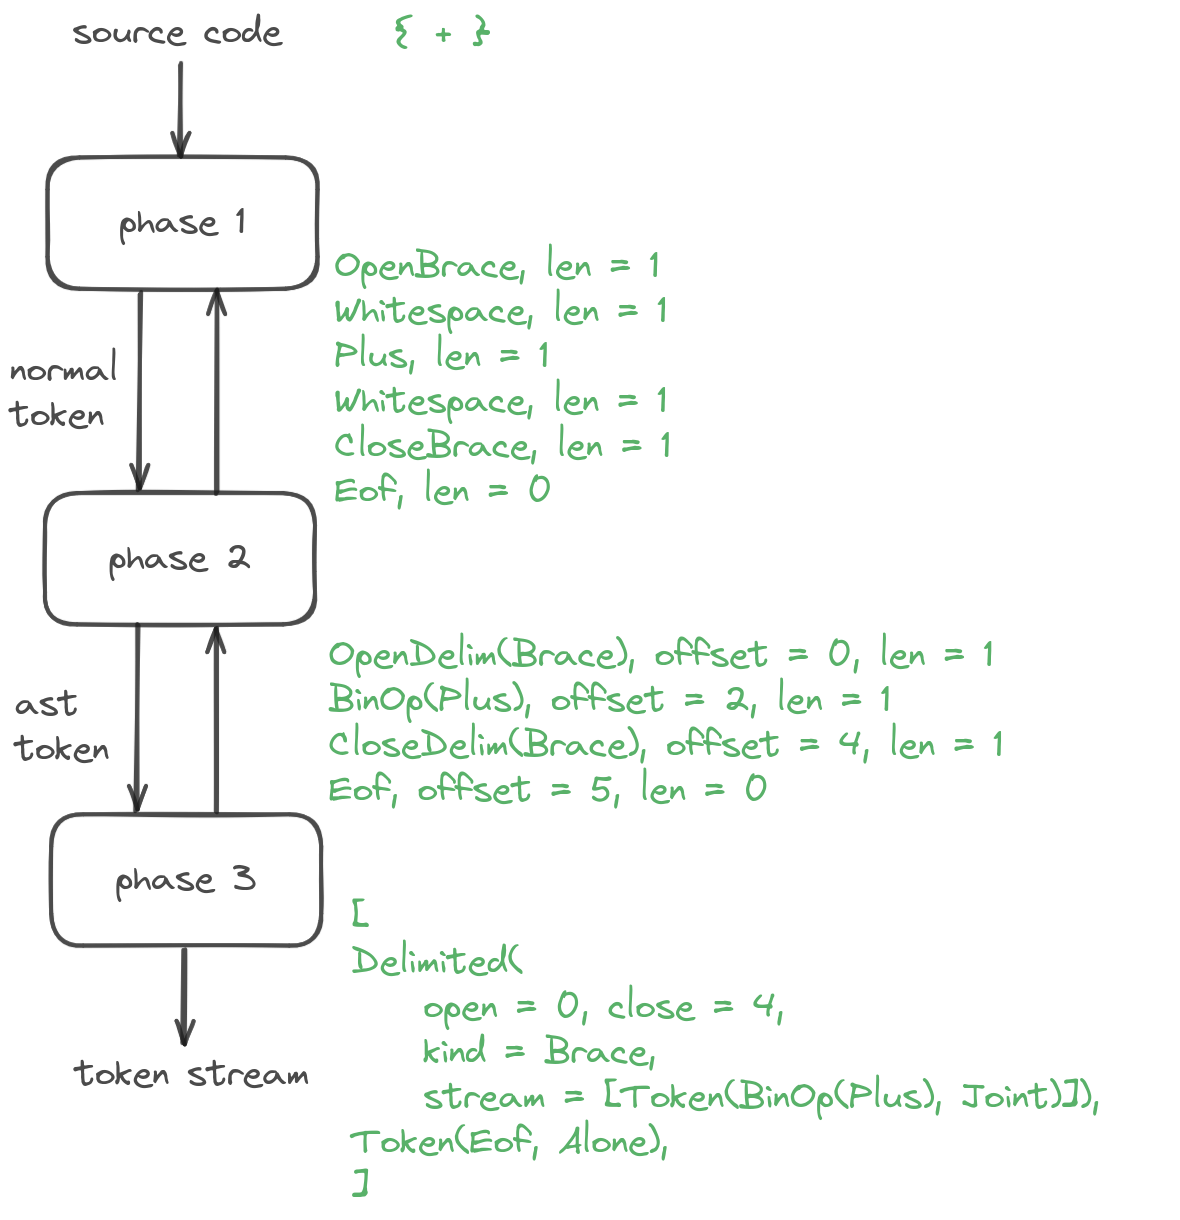
\includegraphics[scale=0.35]{lexer-phases.png}
    \caption{Ba giai đoạn của phân tích từ vựng}
\end{figure}

    Ba giai đoạn của bộ phân tích từ vựng sẽ được trình bày chi tiết như sau:

\subsection{Phân tích từ tố sơ cấp}
    Trong quá trình xây dựng trình thông dịch Pandora, từ tố sơ cấp (Token) là một thành phần quan trọng giúp đại diện cho các đơn vị cơ bản nhất trong mã nguồn, chẳng hạn như từ khóa, toán tử, dấu câu, giá trị số, \dots Mỗi từ tố cần chứa thông tin về loại của nó (kind) và độ dài (len) để hỗ trợ các bước phân tích và thực thi mã nguồn sau này. Cấu trúc của từ tố sơ cấp được thể hiện trong mã nguồn như sau:

\noindent \kw{src/lexer/token.rs}:
\begin{lstlisting}[]
pub struct Token {
    pub kind: TokenKind,
    pub len: u32,
}
\end{lstlisting}

    Ở giai đoạn này, bộ phân tích từ vựng sẽ đọc chương trình nguồn và phân nó thành các loại từ tố khác nhau (TokenKind):

\noindent \kw{src/lexer/token.rs}:
\begin{lstlisting}[]
pub enum TokenKind {
    ...
}
\end{lstlisting}

    Đầu tiên, ta sẽ có các loại từ tố thể hiện các \textbf{ký tự đơn} như \kw{`:`}, \kw{`,`}, \kw{`.`}, \kw{`;`}, ... Dưới đây là đoạn mã về tất cả các loại từ tố ký tự đơn:

\begin{lstlisting}[]
pub enum TokenKind {
    /* one char symbol */
    /// :
    Colon,
    /// ,
    Comma,
    /// .
    Dot,
    /// ;
    Semicolon,
    /// ?
    Question,
    /// (
    OpenParen,
    /// )
    CloseParen,
    /// {
    OpenBrace,
    /// }
    CloseBrace,
    /// [
    OpenBracket,
    /// ]
    CloseBracket,
    /// `!`
    Bang,
    /// `=`
    Eq,
    /// `>`
    Gt,
    /// `<`
    Lt,
    /// `~`
    Tilde,
    /// `+`
    Plus,
    /// `-`
    Minus,
    /// `*`
    Star,
    /// `/`
    Slash,
    /// `%`
    Percent,
    /// `^`
    Caret,
    /// `&`
    And,
    /// `|`
    Or,
    ...
}
\end{lstlisting}

    Tiếp theo, ta sẽ có loại từ tố dành cho các \textbf{chuỗi ký tự}. Ngôn ngữ Pandora hỗ trợ tổng cộng 5 loại chuỗi ký tự: chuỗi, chuỗi thô, số nguyên, số thực và ký tự. Mỗi loại chuỗi sẽ có cấu trúc dữ liệu riêng để lưu trữ thông tin cần thiết. Chẳng hạn, chuỗi thông thường sẽ có thêm thuộc tính \kw{terminated} để xác định xem chuỗi có được đóng đúng cách hay không, còn chuỗi số nguyên sẽ có thêm thuộc tính \kw{base} để xác định hệ cơ số của số nguyên. Trường hợp chuỗi thô thì tương đối là phức tạp. Một chuỗi thô sẽ được đặt trong cặp nháy kép \kw{"} bắt đầu với kí tự \kw{r}. Loại từ tố này có thêm thuộc tính \kw{n\_hashes} để đếm số kí tự \kw{\#} nằm giữa kí tự \kw{r} và \kw{"}. Nếu chuỗi bị sai, \kw{n\_hashes} sẽ mang giá trị \kw{None}. Đối với các chuỗi số thực, thuộc tính \kw{base} sẽ xác định hệ cơ số của số thực, và thuộc tính \kw{empty\_exponent} dùng để xác định xem số nguyên có hợp lệ hay không (phải có phần số mũ sau chữ \kw{e}). Chuỗi ký tự thì khá giống với chuỗi thông thường, với thuộc tính \kw{terminated} để xác định xem ký tự có được đóng đúng cách hay không. Dưới đây là đoạn mã về tất cả các loại từ tố chuỗi:

\begin{lstlisting}[]
pub enum TokenKind {
    ...
    // Literal
    Literal(LiteralKind),
}


pub enum LiteralKind {
    /// `"abc"`, `"ab`, `"ab\"`, `"ab\""`.
    Str {
        terminated: bool,
    },
    /// `r#"abc"#`, `r###"ab"##c"###`, `r###"ab"######`, None means invalid.
    RawStr {
        n_hashes: Option<u8>,
    },
    /// `1_000`, `0b1101`, `0o657`, `0h1af9`.
    Int {
        base: Base,
        empty_int: bool,
    },
    Float {
        base: Base,
        empty_exponent: bool,
    },
    // Although kind can be Char but it can be many symbols (error). Ex: 'abc' -> error.
    /// `'a'`, `'\''`, `'\\'`, `'abc'`, `'ab`.
    Char {
        terminated: bool,
    },
}
\end{lstlisting}

    Loại từ tố tiếp theo là \textbf{tên định danh}. Tên định danh có thể là tên biến, tên hàm, tên kiểu dữ liệu, tên module và từ khóa. Một số ngôn ngữ sẽ phân loại các loại tên này thành các loại từ tố khác nhau. Tuy nhiên, trong Pandora, việc phân loại chúng lại được diễn ra ở giai đoạn phân tích cú pháp. Dưới đây là đoạn mã về loại từ tố định danh:

\begin{lstlisting}[]
pub enum TokenKind {
    ...
    // Identifier
    Ident,
    ...
}
\end{lstlisting}

    Một tính năng khá thú vị của ngôn ngữ Pandora là ngôn ngữ này cho phép người dùng được sử dụng tên trùng với từ khóa. Và để làm được điều này, ta sẽ có một loại từ tố khác, gọi là từ tố \textbf{tên định danh thô}. Tên định danh thô sẽ được phân biệt với tên định danh thông thường thông qua việc thêm kí tự \kw{r\#} vào đầu tên. Dưới đây là đoạn mã về loại từ tố tên định danh thô:

\begin{lstlisting}[]
pub enum TokenKind {
    ...
    // Raw identifier
    RawIdent,
    ...
}
\end{lstlisting}

    Ngoài ra, như bao ngôn ngữ khác, Pandora cũng hỗ trợ các loại từ tố \textbf{chú thích}. Chú thích là một phần không ảnh hưởng đến quá trình thông dịch, nó chỉ được sử dụng để giải thích mã nguồn cho người đọc. Tuy nhiên, Pandora cũng hỗ trợ thêm một loại chú thích đặc biệt, gọi là \textbf{chú thích tài liệu}. Chú thích tài liệu sẽ được sử dụng để tạo ra tài liệu hướng dẫn cho mã nguồn. Loại chú thích này khác với loại chú thích thông thường, nó sẽ không bị bỏ qua trong quá trình phân tích từ vựng. Có hai cách viết chú thích: chú thích trên một dòng và chú thích trên nhiều dòng. Đối với loại chú thích nhiều dòng, Pandora hỗ trợ \textbf{chú thích lồng} (nested comment). Cụ thể về cách viết chú thích ngôn ngữ đã được trình bày ở phần \textbf{\ref{ch2:pandora}}. Dưới đây là đoạn mã về loại từ tố chú thích:

\begin{lstlisting}[]
pub enum TokenKind {
    ...
    // Comments
    LineComment {
        doc_style: Option<DocStyle>,
    },
    BlockComment {
        doc_style: Option<DocStyle>,
        terminated: bool,
    },
    ...
}

pub enum DocStyle {
    Inner,
    Outer,
}
\end{lstlisting}

    Theo đoạn mã trên, ta có thể thấy loại từ tố chú thích sẽ có thêm thuộc tính \kw{doc\_style} để xác định loại chú thích. Nếu thuộc tính này mang giá trị \kw{None}, nghĩa là chú thích này không phải là chú thích tài liệu. Ngược lại, nếu thuộc tính này mang giá trị \kw{Some(DocStyle)}, nghĩa là chú thích này là chú thích tài liệu. Thuộc tính \kw{terminated} sẽ xác định xem chú thích có được đóng đúng cách hay không.

    Trong quá trình viết chương trình, người dùng có thể sẽ sử dụng các khoảng trắng để giúp cho đoạn mã trở nên dễ đọc hơn. Tuy nhiên, các khoảng trắng này không ảnh hưởng đến quá trình thông dịch. Do đó, ta cần có một loại từ tố để biểu diễn các khoảng trắng này. Dưới đây là đoạn mã về loại từ tố \textbf{khoảng trắng}:

\begin{lstlisting}[]
pub enum TokenKind {
    ...
    Whitespace,
    ...
}
\end{lstlisting}

    Những ký tự mà ngôn ngữ Pandora không nhận diện được sẽ được xem là ký tự không hợp lệ, và đều được xếp vào loại từ tố \textbf{không xác định}. Dưới đây là đoạn mã về loại từ tố không xác định:

\begin{lstlisting}[]
pub enum TokenKind {
    ...
    // Unknown token's kind.
    Unknown,
    ...
}
\end{lstlisting}

    Cuối cùng, ta sẽ có loại từ tố \textbf{kết thúc}. Loại từ tố này sẽ được sử dụng để xác định kết thúc của chương trình. Dưới đây là đoạn mã về loại từ tố kết thúc:

\begin{lstlisting}[]
pub enum TokenKind {
    ...
    /// End of input.
    Eof,
    ...
}
\end{lstlisting}

Để có thể xử lý và phân loại các từ tố, ta cần xây dựng một bộ phân tích từ vựng. Bộ phân tích từ vựng sẽ đọc chương trình nguồn và phân tách nó thành các từ tố khác nhau. Việc phân tích này sẽ được thực hiện thông qua hàm \kw{advance\_token} như sau:

\begin{lstlisting}[]
pub fn advance_token(...) -> Token {
    ...
    let first_char = match self.eat() {
        Some(c) => c,
        None => return Token::new(TokenKind::Eof, ...),
    };

    let kind = match first_char {
        c if is_whitespace(c) => self.whitespace(),

        ':' => TokenKind::Colon,
        ',' => TokenKind::Comma,
        '.' => TokenKind::Dot,
        ... // Other single char tokens.

        // Slash, comment or block comment.
        '/' => match self.first() {
            '/' => self.line_comment(),
            '*' => self.block_comment(),
            _ => TokenKind::Slash,
        },

        '0'..='9' => self.number(),

        // Raw identifier, Identifier, Raw double quote string
        'r' => match (self.first(), self.second()) {
            ('#', c1) if is_id_start(c1) => self.raw_identifier(),
            ('#', _) | ('"', _) => {
                let res = self.raw_double_quote_string();
                TokenKind::Literal(LiteralKind::RawStr { n_hashes: res.ok() })
            }
            _ => self.identifier(),
        },

        '\'' => self.single_quote_string(),
        '"' => self.double_quote_string(),

        c if is_id_start(c) => self.identifier(),

        _ => TokenKind::Unknown,
    };

    Token::new(kind, ...)
}
\end{lstlisting}

    Ta có thể thấy, hàm \kw{advance\_token} sẽ trả về một từ tố mới mỗi lần được gọi. Hàm này sẽ đọc từng ký tự trong chương trình nguồn và phân loại chúng thành các loại từ tố khác nhau. Cụ thể, hàm sẽ xử lý các trường hợp sau:

\begin{itemize}
    \item Ký tự khoảng trắng sẽ được chuyển thành từ tố khoảng trắng.
    \item Các ký tự đơn như \kw{`:`}, \kw{`,`}, \kw{`.`}, \kw{`;`}, ... sẽ được chuyển thành các loại từ tố tương ứng.
    \item Ký tự \kw{/} đặc biệt hơn vì có thể là bắt đầu của một chú thích. Ta cần kiểm tra ký tự ngay sau nó để xác định loại từ tố \kw{line\_comment}, \kw{block\_comment} hoặc \kw{Slash}.
    \item Nếu là số, ta sẽ xác định loại từ tố số cụ thể là \kw{Int} hay \kw{Float}, cơ số nào bằng hàm \kw{number}.
    \item Xử lý loại từ tố tên thô và chuỗi thô: nếu ký tự đang đọc là \kw{r}, ta sẽ xác định hai ký tự tiếp theo ngay sau nó. Nếu ký tự tiếp theo là \kw{\#} và sau đó là ký tự bắt đầu tên hợp lệ, ta xác định loại từ tố tên thô bằng hàm \kw{raw\_identifier}; nếu ký tự tiếp theo là \kw{\#} hoặc \kw{"}, ta xác định loại từ tố chuỗi thô bằng hàm \kw{raw\_double\_quote\_string}; trường hợp còn lại, ta xác định loại từ tố tên bằng hàm \kw{identifier}.
    \item Xử lý ký tự: nếu ký tự đang đọc là dấu nháy đơn \kw{'} thì ta xác định loại từ tố ký tự bằng hàm \kw{single\_quote\_string}.
    \item Xử lý chuỗi: nếu ký tự đang đọc là dấu nháy kép \kw{"} thì ta xác định loại từ tố chuỗi bằng hàm \kw{double\_quote\_string}.
    \item Nếu ký tự đang đọc không thỏa mãn bất kỳ trường hợp nào trên thì sẽ là loại từ tố không xác định.
\end{itemize}

Việc xử lý các loại từ tố phức tạp như chuỗi, số, tên định danh, chú thích, ... sẽ được thực hiện thông qua các hàm con. Các hàm này sẽ trả về kết quả tương ứng với loại từ tố cần xác định. Ta sẽ xây dựng các hàm này dựa trên các quy tắc đã định nghĩa trong phần \textbf{\ref{ch2:pandora}} (ta sẽ không đi vào chi tiết các hàm này ở đây).

    Như vậy, ta đã xây dựng xong giai đoạn đầu tiên của quá trình phân tích từ vựng Pandora. Sau khi đã có được các từ tố sơ cấp, ta cần "nâng cấp" chúng thành các từ tố thứ cấp. Các từ tố này sẽ mang nhiều ý nghĩa hơn, và có giá trị hơn cho các giai đoạn sau.

\subsection{Phân tích từ tố thứ cấp}

    Khác với từ tố sơ cấp gồm loại từ tố và độ dài, từ tố thứ cấp cũng có loại từ tố, đi kèm với đó là vị trí chính xác của từ tố này trong đoạn mã chương trình. Việc này sẽ giúp ích rất nhiều trong khâu xử lý lỗi (đã được phân tích kĩ trong phần \textbf{\ref{ch3:err-handler}}). Để lưu được chính xác vị trí, thuộc tính \kw{len} của từ tố sơ cấp đã được thay thế thành thuộc tính \kw{span} với kiểu dữ liệu là \kw{Span}. Struct này gồm có hai thuộc tính là \kw{offset} cho biết vị trí bắt đầu của từ tố trong chuỗi vào, và thuộc tính \kw{length} cho biết chiều dài của từ tố trong chuỗi đầu vào. Chi tiết cấu trúc trên được biểu diễn trong đoạn mã như sau:

\noindent \kw{src/ast/token.rs}:
\begin{lstlisting}
pub struct Token {
    pub kind: TokenKind,
    pub span: Span,
}
\end{lstlisting}

\noindent \kw{src/span\_encoding.rs}:
\begin{lstlisting}
pub struct Span {
    /// The start of the span.
    pub offset: BytePos,
    /// The total length of the span
    pub length: usize,
}
\end{lstlisting}

    Ta cần lưu ý rằng, loại từ tố của từ tố thứ cấp sẽ khác với loại của từ tố sơ cấp. Cụ thể, ngữ nghĩa từ tố sẽ sát với ngôn ngữ hơn. Chẳng hạn, ký tự \kw{!} sẽ được xếp vào loại \kw{Bang} trong từ tố sơ cấp, nhưng khi chuyển sang từ tố thứ cấp, nó lại được gọi là \kw{Not}, tượng trưng cho phép toán phủ định. Việc tổ chức như vậy sẽ giúp giai đoạn phân tích sơ cấp có tính mở rộng, tái sử dụng cực cao, do nó không bị phụ thuộc vào bất kỳ ngữ cảnh ngôn ngữ gì. 

    Các loại từ tố của từ tố thứ cấp sẽ nhiều và đa dạng hơn từ tố sơ cấp. Đầu tiên, một số từ tố loại ký tự đơn đơn giản của bên từ tố sơ cấp sang từ tố thứ cấp không thay đổi gì, như \kw{Colon}, \kw{Comma}, \kw{Dot}, \kw{Semicolon}, ... Tuy nhiên, có một vài từ tố sẽ được thay đổi tên cho sát với ngữ nghĩa hơn, như \kw{Bang} sẽ được đổi thành \kw{Not}. 

    Những loại ký tự đơn tượng trưng cho cặp mở đóng ngoặc như \kw{`\{`}, \kw{`\}`}, \kw{`(`}, \kw{`)`}, \kw{`[`}, \kw{`]`}, ..., khi chuyển sang từ tố thứ cấp sẽ được phân làm hai loại: mở ngoặc và đóng ngoặc (\kw{OpenDelim} và \kw{CloseDelim}). Việc tổ chức như vậy sẽ rất có ích cho việc phân tích thành cây từ tố ở giai đoạn sau. Cụ thể, chúng được thể hiện như sau:

\noindent \kw{src/ast/token.rs}:
\begin{lstlisting}[]
pub enum TokenKind {
    ...
    /// An opening delimiter (e.g., `{`).
    OpenDelim(Delimiter),
    /// A closing delimiter (e.g., `}`).
    CloseDelim(Delimiter),
    ...
}

pub enum Delimiter {
    /// `( ... )`
    Parenthesis,
    /// `{ ... }`
    Brace,
    /// `[ ... ]`
    Bracket,
}
\end{lstlisting}

    Các ký tự đơn được thể hiện dưới dạng dấu toán học đều được xếp vào loại \kw{BinOp} trong từ tố thứ cấp. Điều này sẽ giúp các bộ xử lý sau có thể xác định nhanh chóng các loại từ tố có thể được sử dụng trong các phép toán học. Chúng được biểu diễn theo đoạn mã sau:

\begin{lstlisting}[]
pub enum Token {
    ...
    BinOp(BinOpToken),
    ...
}

pub enum BinOpToken {
    Plus,
    Minus,
    Star,
    Slash,
    Percent,
    Caret,
    And,
    Or,
    Shl,
    Shr,
}
\end{lstlisting}

Các loại chuỗi ký tự đều được tính thành loại \kw{Literal} ở từ tố thứ cấp. Tuy nhiên, mỗi loại chuỗi đều có tên loại của mình \kw{kind} kèm theo nội dung của chuỗi đã được số hóa \kw{symbol}:

\begin{lstlisting}[]
pub enum Token {
    ...
    /* Literals */
    Literal(Lit),
    ...
}

pub struct Lit {
    pub kind: LitKind,
    pub symbol: Symbol,
}

pub enum LitKind {
    Bool,
    Char,
    Int,
    Float,
    Str,
    RawStr(u8), // raw string delimited by `n` hash symbols

    Err,
}
\end{lstlisting}

    Ta để ý rằng từ tố thứ cấp sẽ có thêm một loại chuỗi mới: \kw{Err}. Loại này sẽ được dùng khi quá trình chuyển đổi chuỗi từ từ tố sơ cấp sang từ tố thứ cấp không thành công (chẳng hạn như chuỗi thô có số ký tự \kw{\#} không hợp lệ).

    Cả hai loại tên định danh: tên định danh thông thường và tên định danh thô đều được gộp chung vào loại \kw{Ident} khi chuyển sang từ tố thứ cấp:

\begin{lstlisting}[]
pub enum Token {
    ...
    Ident(Symbol, IdentIsRaw),
    ...
}

pub enum IdentIsRaw {
    Yes,
    No,
}
\end{lstlisting}

    Loại \kw{Ident} trong từ tố thứ cấp sẽ gồm có hai thành phần. Phần thứ nhất là \kw{Symbol} tượng trưng cho chính tên định danh đó đã được số hóa. Phần thứ hai là \kw{IdentIsRaw} cho ta biết được đó là tên định danh thông thường hay tên định danh thô.

    Do các loại khoảng trắng, chú thích không phải tài liệu đều bị bỏ qua, nên từ tố sơ cấp không có loại nào dành cho chúng. Tuy nhiên, từ tố sơ cấp vẫn sẽ có loại cho chú thích tài liệu, cụ thể như sau:

\begin{lstlisting}[]
pub enum Token {
    ...
    /// A doc comment token.
    /// `Symbol` is the data of doc's comment excluding its "quotes" (`///`, `/**`, etc)
    DocComment(CommentKind, Option<DocStyle>, Symbol),
    ...
}

pub enum CommentKind {
    Line,
    Block,
}

pub enum DocStyle {
    Inner,
    Outer,
}
\end{lstlisting}

    Với \kw{CommentKind} sẽ cho biết đó là loại chú thích dòng hay khối. \kw{DocStyle} sẽ cho biết đây là loại chú thích trong hay ngoài. Và \kw{Symbol} sẽ chứa nội dung tài liệu đó.

    Trên cơ sở đó, Ta sẽ xây dựng một hàm để chuyển đổi từng từ tố sơ cấp thành từ tố thứ cấp tương ứng. Quá trình chuyển đổi này còn được gọi là "nấu" từ tố, và được thực hiện thông qua hàm \kw{next\_token}:

\noindent \kw{src/parser/lexer.rs}:
\begin{lstlisting}[]
fn next_token(...) -> Token {
    loop {
        ...
        let token = self.cursor.advance_token();
        let tok_len = token.len;
        let start_pos = self.pos;
        self.pos = self.pos + token.len as BytePos;

        // Now "cook" the token, converting the simple `lexer::TokenKind` to rich `ast::TokenKind`.
        // This also turn strings into interned symbols.
        let kind = match token.kind {
            lexer::TokenKind::LineComment { doc_style } => {
                // Skip normal comment
                let Some(doc_style) = doc_style else {
                    continue;
                };

                ...
                self.cook_doc_comment(..., CommentKind::Line, doc_style)
            }
            lexer::TokenKind::BlockComment {
                doc_style,
                terminated,
            } => {
                ...
                // Skip normal comment
                let Some(doc_style) = doc_style else {
                    continue;
                };

                ...
                self.cook_doc_comment(..., CommentKind::Block, doc_style)
            }
            lexer::TokenKind::Whitespace => {
                continue;
            }
            lexer::TokenKind::Ident => {
                ...
                self.cook_ident(...)
            }
            lexer::TokenKind::RawIdent => {
                ...
                self.cook_raw_ident(...)
            }
            lexer::TokenKind::Literal(kind) => self.cook_literal(..., kind),

            lexer::TokenKind::Eq => TokenKind::Eq,
            lexer::TokenKind::Lt => TokenKind::Lt,
            lexer::TokenKind::Gt => TokenKind::Gt,
            lexer::TokenKind::Bang => TokenKind::Not,
            ... // Other simple tokens.

            lexer::TokenKind::Unknown => {
                self.report_unknown_symbol(...);
                continue;
            }

            lexer::TokenKind::Eof => TokenKind::Eof,
        };

        let span = self.mk_sp(start_pos, self.pos);
        return Token::new(kind, span);
    }

}
\end{lstlisting}

    Trong hàm \kw{next\_token}, ta sẽ lặp qua từng từ tố sơ cấp và chuyển đổi chúng thành từ tố thứ cấp tương ứng. Cụ thể, hàm sẽ xử lý các trường hợp sau:

\begin{itemize}
    \item Nếu từ tố là chú thích dòng và đoạn thông thường (không phải chú thích tài liệu), ta sẽ bỏ qua nó.
    \item Nếu từ tố là khoảng trắng, ta sẽ bỏ qua nó.
    \item Nếu từ tố là tên định danh, ta sẽ chuyển đổi nó thành từ tố tên định danh thứ cấp.
    \item Nếu từ tố là tên định danh thô, ta sẽ chuyển đổi nó thành từ tố tên định danh thô thứ cấp.
    \item Nếu từ tố là chuỗi, ta sẽ chuyển đổi nó thành từ tố chuỗi thứ cấp.
    \item Nếu từ tố là toán tử đơn giản như \kw{=}, \kw{<}, \kw{>}, \kw{!}, ... ta sẽ chuyển đổi nó thành từ tố thứ cấp tương ứng.
    \item Nếu từ tố là từ tố không xác định, ta sẽ báo lỗi.
    \item Nếu từ tố là kết thúc, ta sẽ trả về từ tố kết thúc.
\end{itemize}

    Ta cũng sẽ tính toán vị trí của từ tố trong chuỗi đầu vào và trả về từ tố thứ cấp với thông tin đầy đủ vị trí này. Sau khi đã có được các từ tố thứ cấp, ta sẽ tiến tới việc xây dựng giai đoạn cuối của quá trình phân tích từ vựng: phân tích từ tố thứ cấp thành dãy các cây từ tố.

\subsection{Phân tích cây từ tố}
    Cây từ tố là cấp độ từ tố phức tạp hơn so với hai cấp độ trước. một cây từ tố có thể là một từ tố đơn (lá), hoặc là một nhóm các cây từ tố con được đặt trong cặp đóng mở ngoặc (một cây từ tố con). Điều này được thể hiện qua enum \kw{TokenTree}:

\noindent \kw{src/ast/tokenstream.rs}:
\begin{lstlisting}
pub struct TokenStream(Rc<Vec<TokenTree>>);

pub enum TokenTree {
  /// A single token. Should never be `OpenDelim` or `CloseDelim`, because
  /// delimiters are implicitly represented by `Delimited`.
  Token(Token, Spacing),
  // A delimited sequence of token trees.
  Delimited(DelimSpan, Delimiter, TokenStream),
}

pub enum Spacing {
    Alone,
    Joint,
}

pub struct DelimSpan {
    pub open: Span,
    pub close: Span,
}
\end{lstlisting}

    Cụ thể, một \kw{TokenTree} có thể là một từ tố đơn \kw{Token}. Từ tố này bao gồm hai giá trị: giá trị thứ nhất chính là từ tố thứ cấp của nó (đã được phân tích ở giai đoạn hai), giá trị thứ hai chính là \kw{Spacing}. \kw{Spacing} có hai loại là \kw{Alone} và \kw{Joint}. \kw{Joint} sẽ được sử dụng khi theo sau từ tố là một từ tố dấu cho phép chúng kết hợp được với nhau. Chẳng hạn, nếu ngay sau ký tự \kw{<} là \kw{=} thì chúng có thể kết hợp với nhau tạo thành một từ tố mới là \kw{<=}. Những trường hợp nào không phải \kw{Joint} thì sẽ là \kw{Alone}.

    Đối với loại thứ hai là loại nhóm các cây từ tố con. Các cây từ tố con sẽ được đặt trong cặp ngoặc (\kw{Delimited}). Mỗi cây từ tố thuộc loại này sẽ bao gồm ba giá trị. Đầu tiên là \kw{DelimSpan} giúp xác định chính xác vị trí mở ngoặc và vị trí đóng ngoặc. Tiếp theo là \kw{Delimiter} với vai trò xác định loại của ngoặc đang dùng (ngoặc nhọn, ngoặc tròn, ngoặc vuông). Cuối cùng sẽ là \kw{TokenStream}. Đây là một struct tượng trưng cho một dãy các cây từ tố con.

    Để có thể xây dựng được cây từ tố với cấu trúc như trên, ta sẽ sử dụng hàm \kw{lex\_token\_trees}. Nhiệm vụ của hàm này là chuyển toàn bộ tất cả các từ tố thứ cấp ở giai đoạn thứ hai thành một dãy các cây từ tố con, \kw{TokenStream}:

\noindent \kw{src/parse/lexer.rs}:
\begin{lstlisting}[]
pub fn lex_token_tree<'sess, 'src>(
    ...
) -> PResult<TokenStream> {
    ...
    let (tokenstream, res) = tokentrees::TokenTreesReader::lex_all_token_trees(...);

    if res.is_err() {
        return Err(res.unwrap_err());
    }

    Ok(tokenstream)
}
\end{lstlisting}

\noindent \kw{src/parse/lexer/tokentrees.rs}
\begin{lstlisting}[]
pub fn lex_all_token_trees(
    ...
) -> (TokenStream, PResult<()>) {
    let mut tt_reader = TokenTreesReader {...};
    tt_reader.lex_token_trees(false)
}

fn lex_token_trees(..., is_delimited: bool) -> (TokenStream, PResult<()>) {
    ...
    let mut buf = Vec::new();
    loop {
        match self.token.kind {
            TokenKind::OpenDelim(delim) => match self.lex_token_tree_open_delim(delim) {...},
            TokenKind::CloseDelim(delim) => {
                if !is_delimited {
                    let err = PError::UnexpectedClosingDelimiter {...};
                    return (TokenStream::new(buf), Err(vec![err]));
                }
                return (TokenStream::new(buf), Ok(()));
            }
            TokenKind::Eof => {
                if is_delimited {
                    ...
                    let err = PError::UnclosedDelimiter {...};
                    return (TokenStream::new(buf), Err(vec![err]));
                }
                return (TokenStream::new(buf), Ok(()));
            }
            _ => {
                ...
                match this_tok.kind {
                    _ => {
                        buf.push(TokenTree::Token(...));
                    }
                }
            }
        }
    }
}
\end{lstlisting}

    Ta có thể thấy, luồng logic chính sẽ nằm trong hàm \kw{lex\_token\_tree}. Một tham số quan trọng của hàm này là \kw{is\_delimited} dùng để xác định xem loại cây từ tố đang xét là loại nào. Hàm này sẽ trả về cây từ tố kèm theo kết quả cho biết cây đó có hợp lệ hay không. Trong quá trình xét các từ tố thứ cấp, có bốn trường hợp có thể xảy ra:

\begin{itemize}
    \item Nếu từ tố đang đọc được là dấu mở ngoặc, ta sẽ bắt đầu đoán nhận một cây từ tố loại \kw{Delimited}. Loại này sẽ được xử lý thông qua hàm \kw{lex\_token\_tree\_open\_delim}
    \item Nếu từ tố đang đọc được là dấu đóng ngoặc, tuy nhiên cây từ tố đang xét không thuộc loại \kw{Delimited}, hàm sẽ báo lỗi và kết thúc vòng lặp. Trường hợp ngược lại, hàm sẽ kết thúc và trả về dãy cây từ tố đó.
    \item Nếu từ tố là từ tố kết thúc, tuy nhiên cây từ tố đang xét lại thuộc loại \kw{Delimited}, hàm cũng sẽ báo lỗi và kết thúc vòng lặp. Trường hợp ngược lại, hàm sẽ kết thúc và trả về dãy cây từ tố đó.
    \item Với những từ tố thông thường khác, hàm sẽ đẩy từ tố đó vào dãy và tiếp tục vòng lặp. 
\end{itemize}

    Đối với trường hợp từ tố đọc được là dấu mở ngoặc, như đã phân tích ở trên, ta sẽ sử dụng hàm \kw{lex\_token\_tree\_open\_delim} để phân tích. Đoạn mã của hàm này sẽ được thể hiện như sau:

\begin{lstlisting}[]
fn lex_token_tree_open_delim(..., open_delim: Delimiter) -> PResult<TokenTree> {
    ...
    let (tts, res) = self.lex_token_trees(/* is_delimited */ true);
    if res.is_err() {
        return Err(res.unwrap_err());
    }

    ...
    match self.token.kind {
        // Correct delimiter.
        TokenKind::CloseDelim(close_delim) if close_delim == open_delim => {
            ...
        }

        // Incorrect delimiter.
        TokenKind::CloseDelim(close_delim) => {
            let err = PError::MismatchedClosingDelimiter {...};
            return Err(vec![err]);
        }
        TokenKind::Eof => {}
        _ => unreachable!(),
    }

    Ok(TokenTree::Delimited(...))
}
\end{lstlisting}

    Hàm này sẽ nhận một tham số quan trọng là \kw{open\_delim} để biết được loại mở ngoặc đang dùng là loại nào (ngoặc vuông, ngoặc nhọn hay ngoặc tròn). Hàm sẽ trả về cây từ tố nếu thành công, ngược lại sẽ trả về lỗi. Đầu tiên, hàm sẽ thực hiện gọi đệ quy hàm \kw{lex\_token\_tree} (đã được phân tích phía trên) để xác định toàn bộ dãy cây từ tố con có bên trong cặp đóng mở ngoặc. Nếu kết quả nhận được là lỗi, hàm sẽ ngay lập tức trả về lỗi đó. Nếu không, ký tự tiếp theo được xét sẽ phải là dấu đóng ngoặc cùng loại với dấu mở ngoặc trước đó. Trường hợp hai dấu mở đóng ngoặc không cùng loại hay không bắt gặp dấu đóng ngoặc, hàm đều trả về lỗi. Còn nếu mở đóng ngoặc khớp với nhau thì đây là loại cây từ tố \kw{Delimited} hợp lệ và hàm sẽ trả về cây từ tố đó.

    Trải qua ba giai đoạn phân tích từ tố phức tạp, ta đã thu được một cây từ tố với đầy đủ các thông tin hữu ích, giúp cho các khối xử lý tiếp sau sẽ dễ dàng phân tích, xử lý hơn. Tiếp theo đây, ta sẽ tiến tới phần tiếp theo, đó chính là công cuộc xây dựng bộ phân tích cú pháp.
